%qqqqqqqqqqqqqqqqqqqqqqqqqqqqqqqqqqqqqqqqqqqqqqqqqqqqqqqqqqqqqqqqqqqqqqqqq
%Quote
\begin{savequote}[50mm]
‘‘Lo más incomprensible de nuestro universo es que sea comprensible’’
\qauthor{Albert Einstein}
\end{savequote}
%qqqqqqqqqqqqqqqqqqqqqqqqqqqqqqqqqqqqqqqqqqqqqqqqqqqqqqqqqqqqqqqqqqqqqqqqq




%#########################################################################
\chapter{El Entorno Cosmológico y el Grupo Local}
\label{cha:Results}


A continuación son presentados los resultados obtenidos a partir de las 
simulaciones descritas en el capítulo anterior \ref{cha:N-BodySimulations} 
para la dependencia de las propiedades de los sistemas tipo grupo 
local respecto al entorno cosmológico en el que están embebidos. Se 
caracteriza primero cada una de las simulaciones usadas (CLUES y Bolshoi) 
con el fin de garantizar concordancia entre las cosmologías que representan 
y entre las distribuciones de entorno (sección 
\ref{sec:StatisticalPropertiesOfAllSimulations}). Después de esto, en la
sección \ref{sec:PropertiesOfSamplePairs} se determinan las propiedades 
físicas y estadísticas de cada una de las muestras definidas en 
\ref{subsec:SampleOfPairsToUse} y se analizan las correlaciones 
existentes entre las propiedades calculadas y el entorno cosmológico de 
cada simulación.


%#########################################################################




%*************************************************************************
%Statistical properties of all simulations
\section{Propiedades de las Simulaciones}
\label{sec:StatisticalPropertiesOfAllSimulations}


Uno de los principales objetivos para determinar la influencia del entorno
sobre sistemas tipo grupo local es construir una muestra \textit{CLG} 
en simulaciones no res\-tringidas y así obtener estadística significativa. 
Para garantizar la consistencia de esta muestra es necesario
establecer la equivalencia entre las entre las distribuciones de halos 
oscuros y analizar las distribuciones de entorno cosmológico para cada 
simulación.


	%---------------------------------------------------------------------
	%Halos Properties
	\subsection{Función de Masa de los Halos}
	\label{subsec:Halos_Properties}
	%---------------------------------------------------------------------


La distribución espacial de los halos refleja la fina estructura de la red 
cósmica formada por la materia oscura, tanto en simulaciones (ver figura 
\ref{fig:Halos_Web}) como en observaciones cosmológicas (ver sección 
\ref{sec:CosmologicalObservations}). Esto sugiere posibles correlaciones 
entre las propiedades de los halos y el entorno en el cual están embebidos, 
tal como es mostrado para la forma de los halos, el parámetro de espín y 
alineación de subhalos en \cite{libeskind2013}, y para la masa de los halos 
\cite{lemson1999}. En especial el trabajo de \cite{libeskind2013} demuestra 
que el esquema de clasificación V-web es el más apropiado para estudios de 
correlaciones con propiedades direccionales, tal como el momento angular de 
los sistemas \textit{IP} o \textit{CLG} en la sección
\ref{sec:PropertiesOfSamplePairs}.

\
%.........................................................................
%FOF method in CLUES simulation
\begin{figure}[htbp]
	\centering
	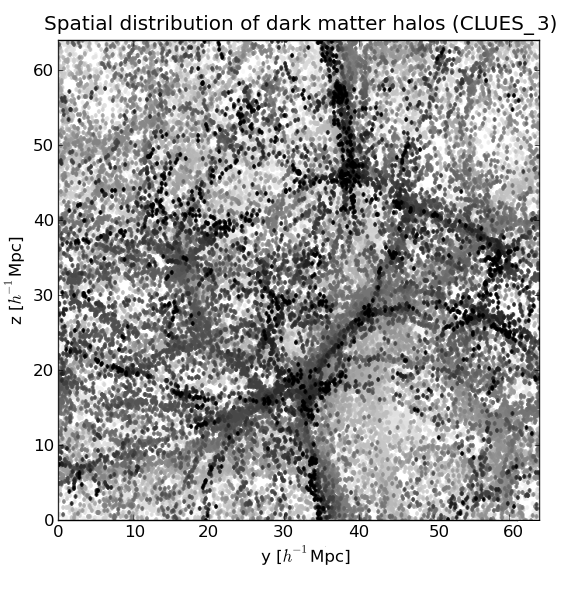
\includegraphics[width=0.62\textwidth]
	{./figures/3_nbody_simulations/Halos_Spatial_Distribution(CLUES_16953).png}

	\caption{\small{Distribución espacial de los halos de materia oscura, 
	reflejando la estructura de la red cósmica. El gradiente de color 
	indica la profundidad respecto al eje $x$, donde los halos negros son 
	los más cercanos.}}
	
	\label{fig:Halos_Web}
\end{figure}
%.........................................................................


Acorde a las condiciones definitorias de las muestras \textit{IP} y 
\textit{CLG} presentadas en la subsección \ref{subsec:SampleOfPairsToUse}, 
la principal propiedad de los halos necesaria para la construcción de estas 
muestras es la masa. Por esta razón es importante establecer la equivalencia 
entre las distribuciones de masa en cada simulación. En la siguiente figura 
\ref{fig:IMF} se calculan las funciones integradas de masa para la simulación 
Bolshoi y para las tres simulaciones CLUES.


%.........................................................................
%Integrated Mass Fraction
\begin{figure}[htbp]
	\centering
	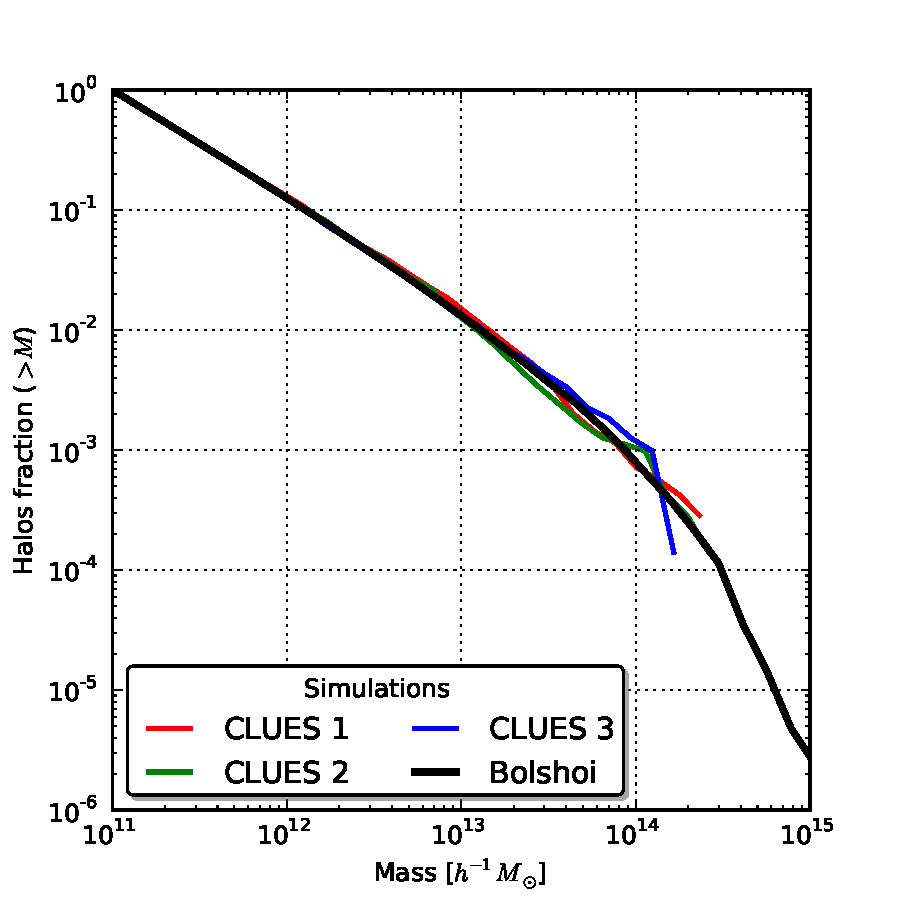
\includegraphics[width=0.70\textwidth]
	{./figures/4_results/Halos_IMF.pdf}
	
	\caption{\small{Funciones de masa integrada de halos de materia oscura 
	(muestra GH) para cada simulación.}}
	\label{fig:IMF}
\end{figure}
%.........................................................................


Para valores de masa altos las distribuciones son ligeramente diferentes 
debido a la menor cantidad de datos en las simulaciones CLUES, lo que hace
menos significativa la estadística en este caso. A pesar de esto, en el
rango masa donde son definidas las muestras \textit{IH} 
($5.0 \times 10^{11}\Msun - 5.0\times 10 ^{12}\Msun$) las distribuciones 
son consistentes con el formalismo Press-Schechter \cite{press1974} para 
los parámetros cosmológicos WMAP7, indicando así la equivalencia de las 
muestras definidas entre las simulaciones.


	%---------------------------------------------------------------------
	%Environment Properties
	\subsection{Distribución del Entorno Cosmológico}
	\label{subsec:Environment_Properties}
	%---------------------------------------------------------------------


Como fue mostrado en la sección \ref{sec:EnvironmentCharacterization}, 
la caracterización del entorno cosmológico se logra a partir de cantidades
físicas que indiquen el carácter geométrico o dinámico local de una región
de la distribución de materia. En especial el esquema V-web permite dar 
cuenta de la dinámica a pequeñas escalas de la estructura de la red cósmica,
permitiendo definir un entorno adecuado para los halos y otros sistemas.
En la siguiente figura son calculadas las distribuciones para cada uno de 
los autovalores de la V-web (distribuciones de entorno), tanto para las 
celdas de las simulaciones, como para los entornos de los halos de la 
muestra \textit{GH}.


%.........................................................................
%1D Distribution of Vweb eigenvalues in cells
\begin{figure}[htbp]
	\centering
	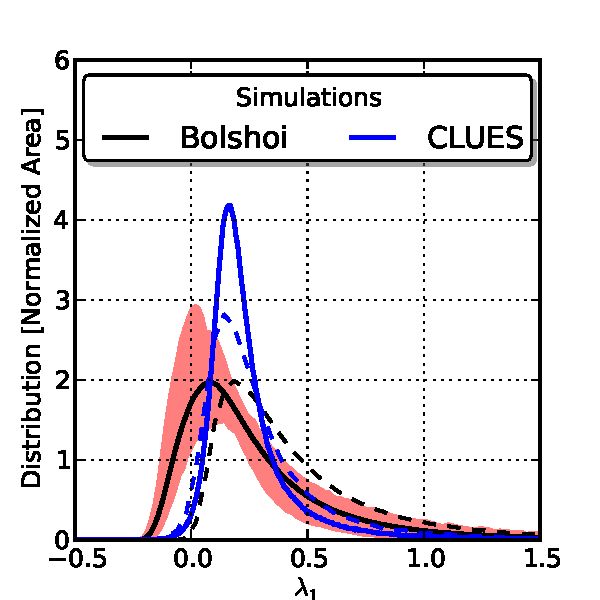
\includegraphics[width=0.4\textwidth]
	{./figures/4_results/Cells_Distro_L1.pdf}
	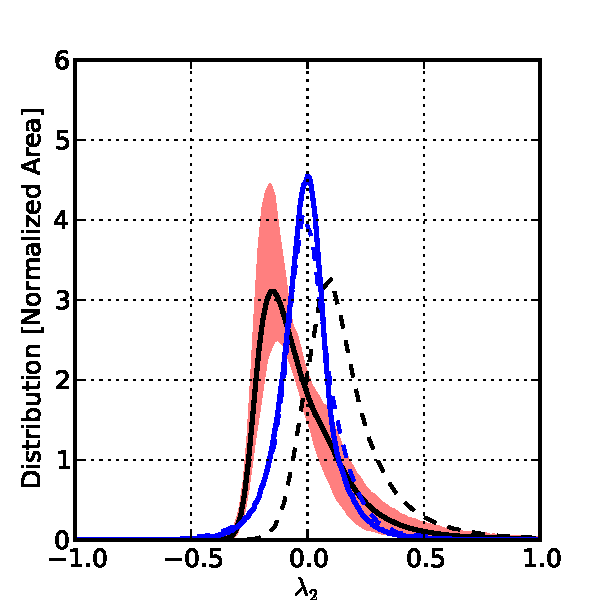
\includegraphics[width=0.4\textwidth]
	{./figures/4_results/Cells_Distro_L2.pdf}
	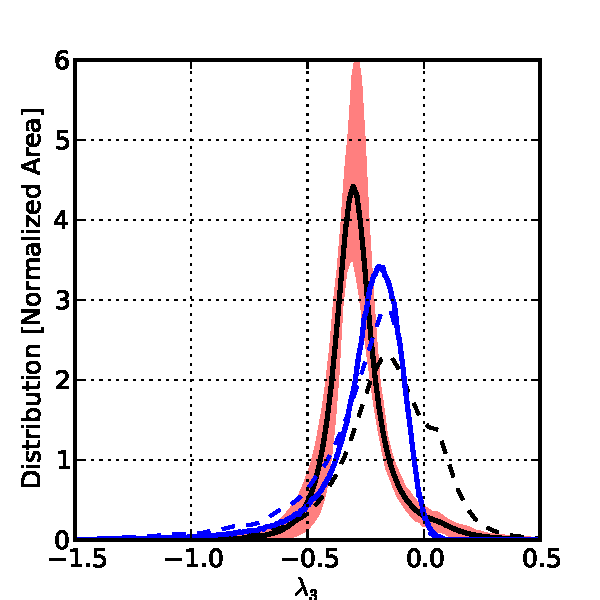
\includegraphics[width=0.4\textwidth]
	{./figures/4_results/Cells_Distro_L3.pdf}

	\caption{\small{ Distribución de los autovalores en el esquema V-web
	para cada una de las celdas de volumen (línea continua) y para los 
	entornos de los halos de materia oscura en los catálogos FOF (línea 
	discontinua). Las distribuciones están normalizadas tal que su área es
	la unidad. Resolución de $1.0 h^{-1}$ Mpc/celda y suavizado Gaussiano
	de una celda.}}
	\label{fig:1D_Cells_Eigenvalues}
\end{figure}
%.........................................................................


El principal resultado de la figura \ref{fig:1D_Cells_Eigenvalues} consiste 
en la diferencia de las distribuciones para las celdas de volumen (líneas 
continuas) entre la simulación Bolshoi y las simu\-laciones CLUES
\footnote{Debido a la alta semejanza entre las distribuciones de las tres
simulaciones CLUES, y con el fin de obtener estadística más significativa,
se han fusionado las distribuciones.}. El efecto de varianza cósmica 
(regiones rojas) es incluido a partir del cálculo de distribuciones de 
entorno en $64$ subvolúmenes de la simulación Bolshoi, con un tamaño similar 
a una simulación CLUES. A pesar de esto, las distribuciones de CLUES están 
por fuera de la región de varianza cósmica, indicando así una estructura 
cosmológica a gran escala que difiere entre ambas simulaciones.


Un segundo resultado importante de la figura \ref{fig:1D_Cells_Eigenvalues}
se obtiene a partir de las distribuciones de entorno para los halos 
(líneas discontinuas). En el caso de Bolshoi, se nota un importante
sesgo entre la distribución de entorno de las celdas y de los halos, 
indicando así que la distribución espacial de los halos no es un buen 
trazador de la estructura a gran escala del campo de densidad. Este 
resultado es consistente con el trabajo de \cite{libeskind2013}, donde 
hallan importantes sesgos en las distribuciones de entorno acorde a 
diferentes rangos de masa de los halos, también usando Bolshoi. En el 
caso de las simulaciones CLUES, las distribuciones de entorno de los 
halos son significativamente menos sesgadas respecto a las de celdas de 
volumen, indicando para este caso que los halos si se distribuyen 
espacialmente acorde al entorno cosmológico cuantificado por el esquema 
V-web.


Por último, en la figura \ref{fig:Vol_Fraction} son calculadas las 
densidades medias y las fracciones de volumen para cada uno de los tipos 
de regiones (ver sección \ref{sec:EnvironmentCharacterization}) acorde al 
valor umbral $\lambda_{th}$. Las funciones de fracción de volumen son 
diferentes entre las simulaciones CLUES y Bolshoi, en especial la región 
en torno a $\lambda_{th} = 0.1$ para las regiones tipo hoja (sheet). Esto se 
debe al desplazamiento relativo entre los picos de las distribuciones de 
entorno para cada simulación (ver figura \ref{fig:1D_Cells_Eigenvalues}), 
lo que implica un comportamiento diferente al criterio de selección de 
regiones a partir del valor $\lambda_{th}$. A pesar de esto, las fracciones 
de volumen se mantienen más o menos consistentes para ambas simulaciones 
en el rango  $0.2 \leq \lambda_{th} \leq 0.4$, que corresponde al rango 
donde mejor se reproduce visualmente la distribución global del campo de 
densidad.

\newpage
%.........................................................................
%Volume Fraction
\begin{figure}[htbp]
	\centering
	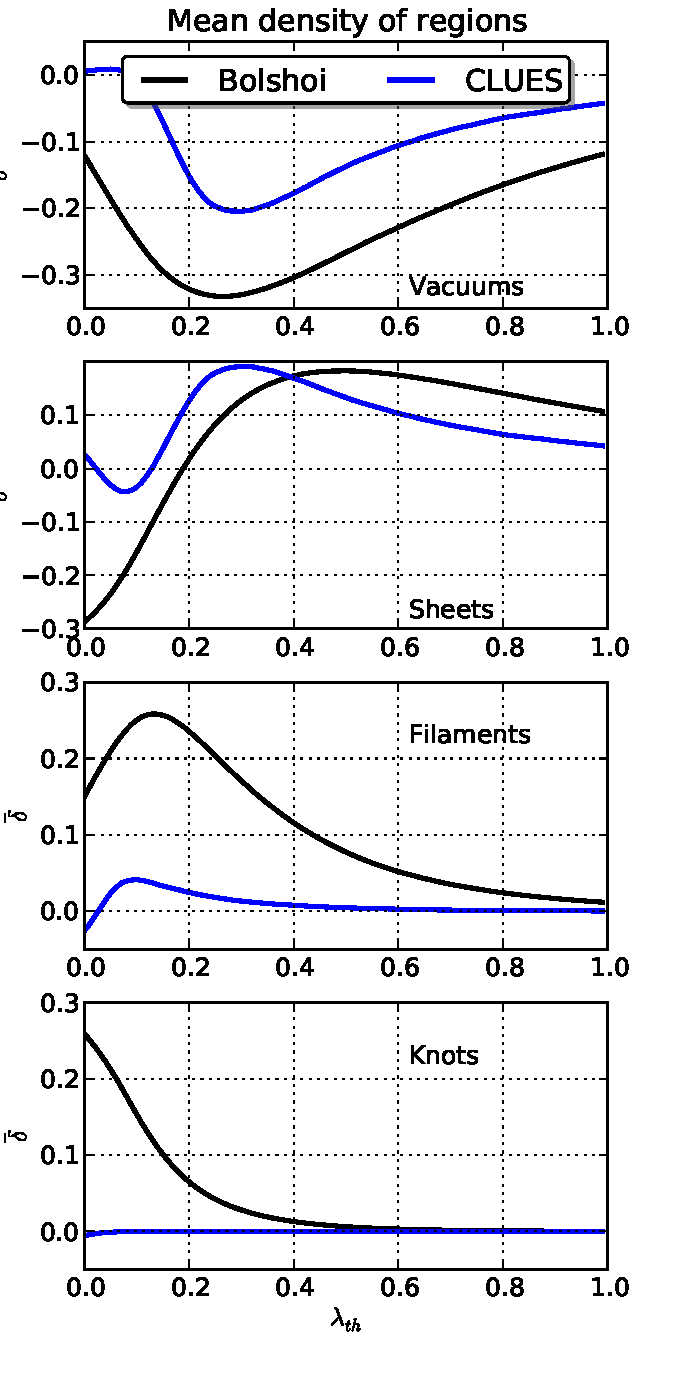
\includegraphics[width=0.43\textwidth]
	{./figures/4_results/Density_Regions.pdf}
	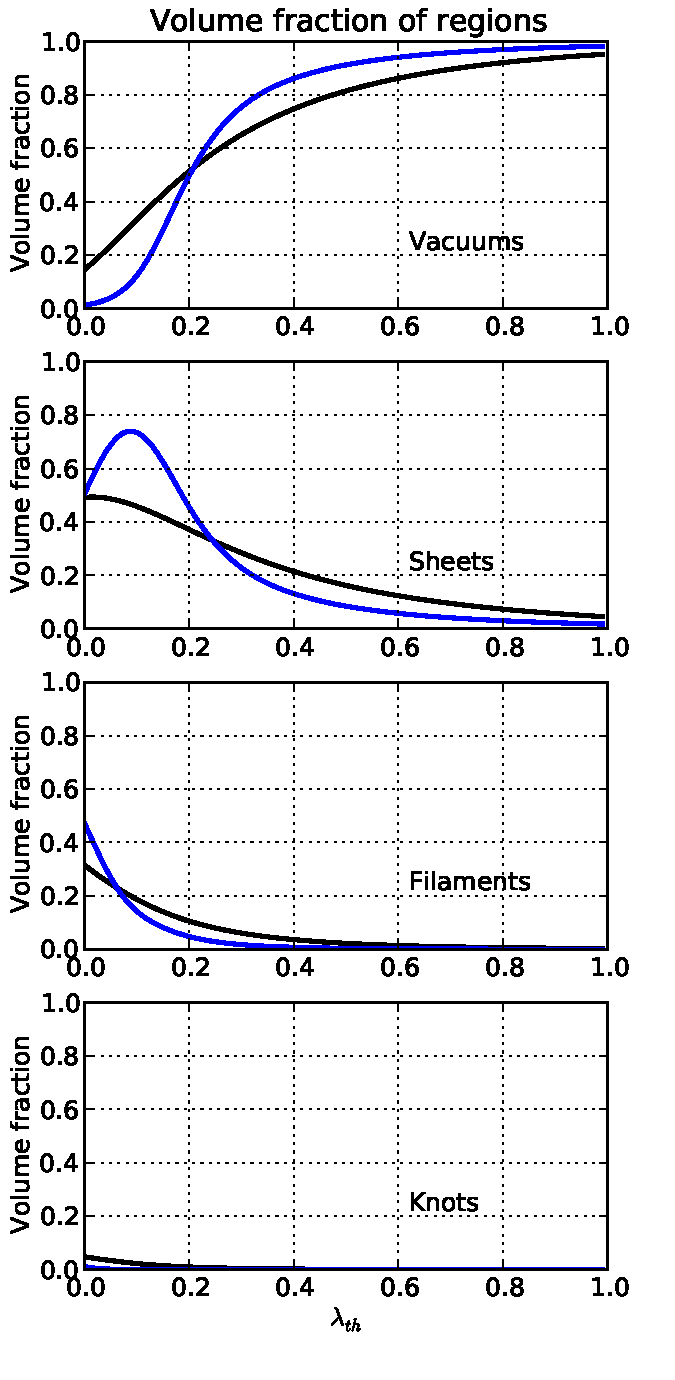
\includegraphics[width=0.43\textwidth]
	{./figures/4_results/Volume_Regions.pdf}
	
	\caption{\small{Parámetro de densidad medio para diferentes tipos
	de regiones en función del valor umbral $\lambda_{th}$ (paneles 
	izquierda). Fracciones de volumen normalizadas para diferentes tipos
	de regiones, también acorde al valor umbral $\lambda_{th}$.}}
	\label{fig:Vol_Fraction}
\end{figure}
%.........................................................................


Las gráficas de densidad media para cada tipo de región muestran 
importantes resultados respecto al entorno cosmológico. Lo primero que 
puede notarse es la diferencia entre las densidades medias de ambas 
simulaciones en cada una de las regiones. Por ejemplo para regiones de 
vacío, en Bolshoi estas corresponden a zonas con densidad promedio mucho 
menor a la densidad media de la simulación, mientras que para las CLUES 
estas zonas de subdensidad no son tan marcadas. Debido a la pequeña 
fracción de volumen de las regiones tipo nudo (knot) en ambas 
simu\-laciones, asociado a su dimensionalidad puntual, la estructura 
global del entorno puede entenderse bien solo en términos de la 
distribución espacial de vacíos, hojas y filamentos, siendo los 
filamentos la contraparte de los vacíos respecto al parámetro de densidad. 
De esto se espera que la diferencia en la subdensidad de los vacíos entre
cada simulación se extienda a una marcada diferencia entre las 
sobredensidades de los filamentos en cada simulación. Esto último es 
obtenido en la misma figura, donde puede verse que los filamentos de 
Bolshoi son notablemente más densos que aquellos de las CLUES. En el caso
de las hojas, estas corresponden a regiones de densidad intermedias entre
los filamentos y los vacíos, por tanto se espera que la diferencia de
la densidad media de estas regiones no sea tan marcada entre ambas 
simulaciones, tal como se nota en la misma figura.


%.........................................................................
%Vweb Comparison
\begin{figure}[htbp]
	\begin{center}
	\makebox[\textwidth]{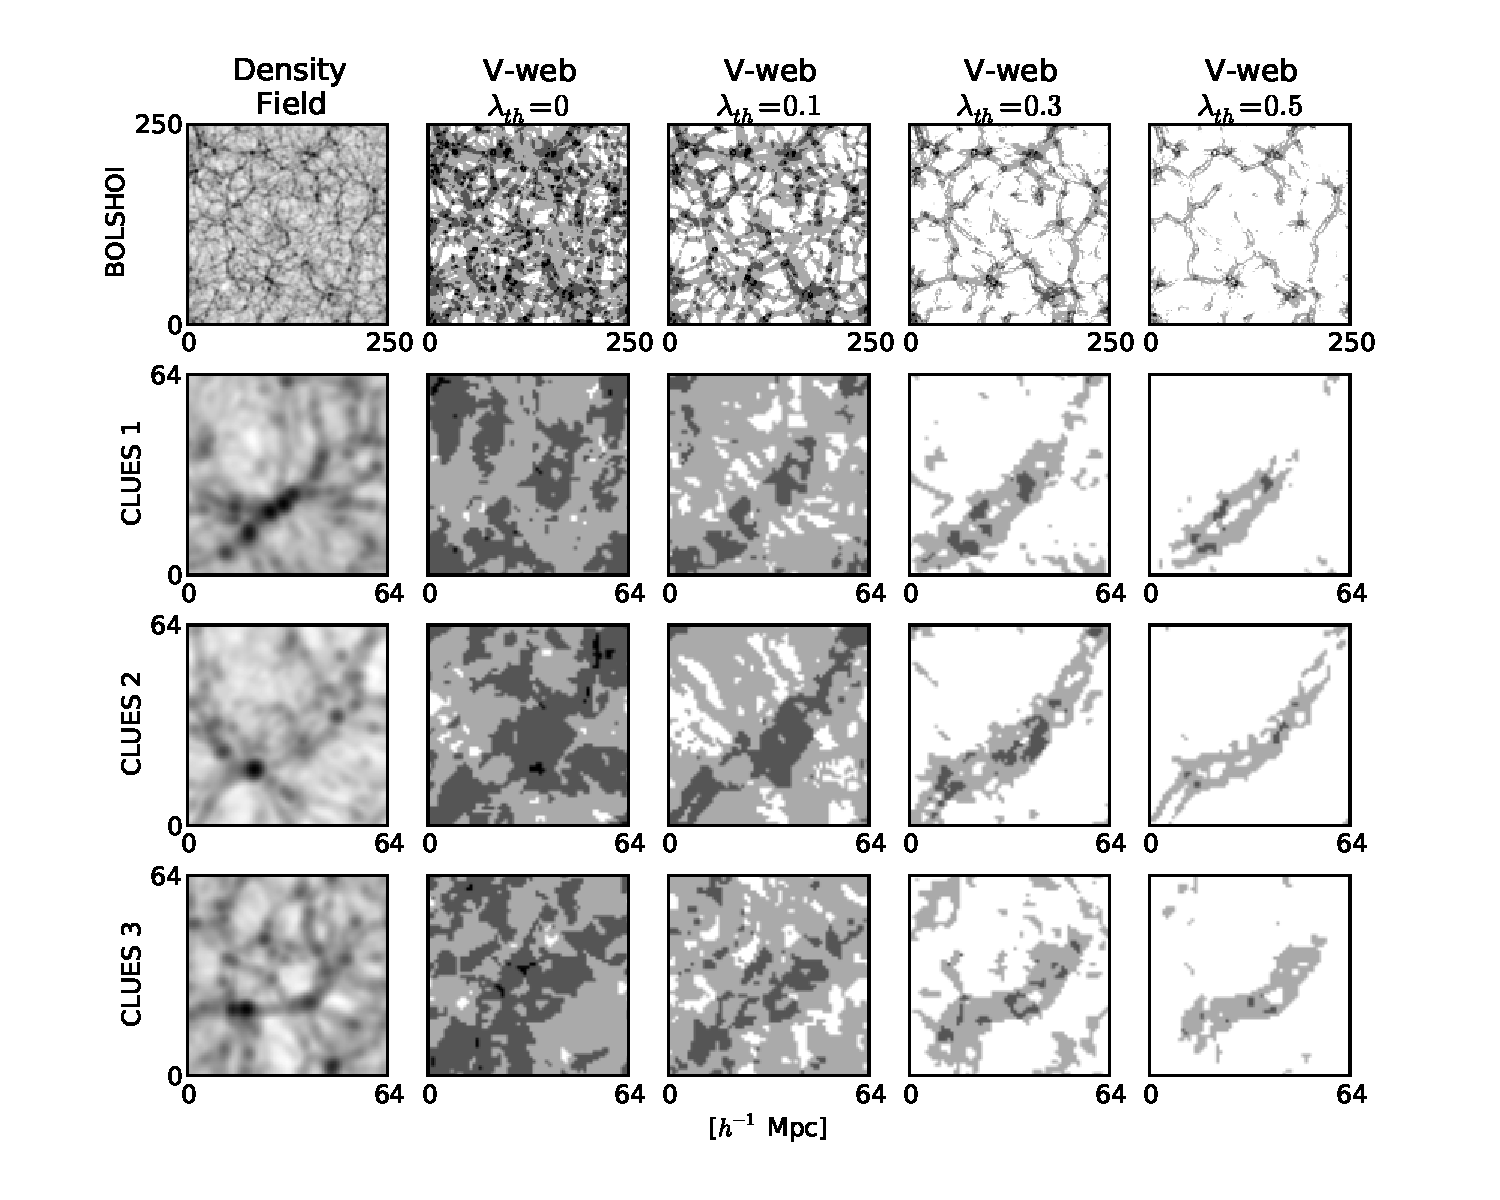
\includegraphics[trim = 10mm 10mm 10mm 9mm, clip,
	width=0.66\paperwidth,angle=0]
	{./figures/4_results/Vweb_Comparison.pdf}}
	\end{center}	
	
	\caption{\small{Comparación de la impresión visual obtenida con el  
	método V-web para varios valores del parámetro $\lambda_{th}$.
	Se usa el siguiente esquema de clasificación (Negro - Nudo, Gris 
	oscuro - Filamento, Gris - Hoja, Blanco - Vacío). La resolución de 
	cada malla es $1.0 h^{-1}$ Mpc/celda, con un suavizado Gaussiano de 
	una celda. El grosor de cada slide es de una celda.}}
	\label{fig:Vweb_Comparison}
\end{figure}
%.........................................................................


Un segundo resultado de la figura \ref{fig:Vol_Fraction} consiste en la 
determinación de un parámetro $\lambda_{th}$ óptimo para la reproducción 
visual de la red cósmica. Como se muestra en esta gráfica, las fracciones
de volumen asociadas a vacíos y hojas son relativamente altas respecto a 
las de filamentos y nudos, esto para todo el rango barrido de valores de 
$\lambda_{th}$. De esto se espera que la impresión visual a gran escala
del campo de materia sea completamente dominada por la distribución de 
vacíos y en menor medida por la distribución de hojas y filamentos. En el 
caso de un valor bajo del parámetro $\lambda_{th}$, por ejemplo 
$\lambda_{th}<0.2$, el parámetro de densidad media de las hojas es negativo, 
indicando que posiblemente estas regiones están invadiendo zonas que deberían 
ser vacíos, tal como se ve en la figura \ref{fig:Vweb_Comparison} para 
$\lambda_{th} = 0$ o $\lambda_{th} = 0.1$. En el caso de valores altos, 
$\lambda_{th} > 0.4\sim 0.5$, el parámetro de densidad medio para los vacíos 
comienza a aumentar, indicando que estas regiones están invadiendo zonas
que de mayor densidad, que en principio deberían ser hojas o filamentos. 
Esto puede ser notado en la figura \ref{fig:Vweb_Comparison} para 
$\lambda_{th} = 0.5$, donde todo el volumen es ampliamente dominado por 
vacíos, perdiendo la estructura característica de la red cósmica. Este 
análisis sugiere que el valor óptimo de $\lambda_{th}$ podría ser aquel 
donde se minimice la densidad media de los vacíos, al ser estos el entorno
dominante. Un resultado que apoya este criterio es que el $\lambda_{th}$ 
encontrado es similar para ambas simulaciones $\lambda_{th}\approx 0.3$,
y coincide con el valor obtenido a partir de un análisis cualitativo de 
la impresión visual del entorno.

\

Para concluir esta sección se discuten los resultados obtenidos para las 
distribuciones de entorno. A pesar de existir un notable sesgo entre
la distribución de los halos y la del campo de densidad en la simulación 
Bolshoi, caso contrario a las simulaciones CLUES, y haber una marcada 
diferencia entre las densidades medias de las regiones en ambas 
simulaciones, la esencia de construir una muestra \textit{CLG} en la 
simulación Bolshoi a partir de los grupos locales de las CLUES, como se 
menciona en el capítulo \ref{cha:N-BodySimulations}, es obtener una muestra 
de pares aislados más fiel que también reproduzcan el entorno local de los 
\textit{LG}. Se espera entonces que la dinámica local cuantificada por la 
V-web se independiente del diferente resultado global de las distribuciones,
manteniéndose así la validez del esquema de construcción de los \textit{CLG}.


%*************************************************************************




%*************************************************************************
%Properties of sample pairs
\section{Propiedades de la Muestra \textit{CLG}}
\label{sec:PropertiesOfSamplePairs}


Una vez determinada la consistencia entre las muestras definidas en CLUES
y Bolshoi, el siguiente paso es determinar sus propiedades. Es de especial
interés analizar la muestra \textit{CLG} de Bolshoi, tomando como muestra 
de control la \textit{IP} y como muestra de referencia la \textit{LG} de 
las simulaciones CLUES.


	%---------------------------------------------------------------------
	%Determination of their host environment
	\subsection{Determinación del Entorno}
	\label{subsec:DeterminationOfTheirHostEnvironment}
	%---------------------------------------------------------------------

Como fue definido en la subsección \ref{subsec:SampleOfPairsToUse} del 
capítulo pasado, la muestra \textit{CLG} en la simulación Bolshoi se 
construye imponiendo a la muestra \textit{IP} la condición extra de 
reproducir el entorno cosmológico de los grupos locales de las simulaciones 
CLUES. La principal motivación de esto es encontrar una muestra en Bolshoi 
análoga a las muestras \textit{LG}, tanto en sus propiedades físicas 
como en su abundancia. Respecto a esto último es natural asumir, 
considerando la ya determinada consistencia entre las simulaciones, que la 
abundancia escala aproximadamente como el volumen simulado. Esto puede 
ser considerado el primer logro de este esquema, ya que reproduce 
aproximadamente esta ley de escalamiento para el tamaño de las muestras 
en cuestión (ver tabla \ref{tab:Samples} para \textit{CLG} de Bolshoi y
\textit{LG} de CLUES).


A pesar de lo anterior, este método de construcción no es más que corte
de la muestra \textit{IP} respecto a los autovalores de la V-web de la 
celda donde están embedidos, lo cual no implica la reproducción 
adecuada de las propiedades físicas ni el entorno cosmológico de los 
sistemas tipo grupo local. Por esta razón, a conti\-nuación son analizados
posibles sesgos producidos en las distribuciones del entorno cosmológico
para los sistemas \textit{CLG}.

	
%.........................................................................
%Pathogenic Situation
\begin{figure}[htbp]
	\centering
	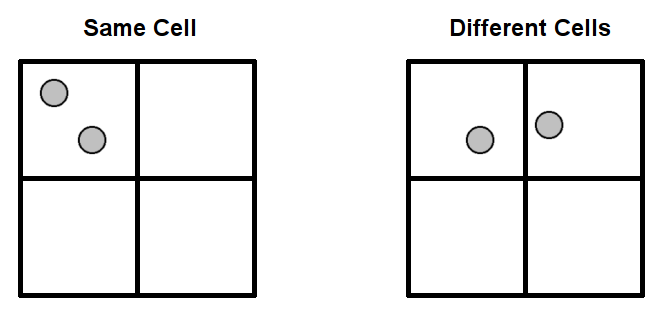
\includegraphics[width=0.5\textwidth]
	{./figures/4_results/Pathogenic_Situation.png}
	
	\caption{\small{Situación patológica respecto al entorno de los sistemas
	de pares de halos.}}
	\label{fig:Pathogenic_Situation}
\end{figure}
%.........................................................................


Una de las primeras consideraciones que debe tenerse en cuenta en la 
cuantificación del entorno para pares de halos (muestras \textit{P}, 
\textit{IP}, \textit{CLG} y \textit{LG}), es que cada uno de ellos puede 
estar embebido en celdas diferentes, tal como es mostrado en la figura 
\ref{fig:Pathogenic_Situation}. Esta situación patológica se presenta debido 
al carácter no puntual de este tipo de sistemas y el tamaño finito de la malla.

\
%.........................................................................
%Comparison of Lambda in each Halos of Pairs systems
\begin{figure}[htbp]
	\centering
	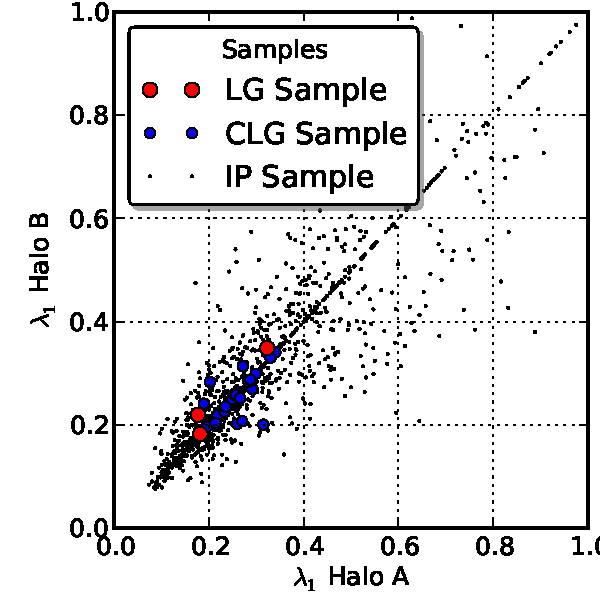
\includegraphics[width=0.46\textwidth]
	{./figures/4_results/CLG_L11_L12.pdf}
	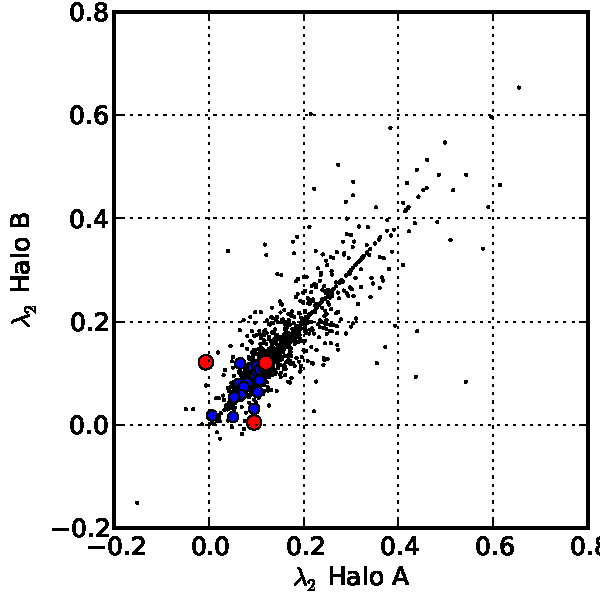
\includegraphics[width=0.46\textwidth]
	{./figures/4_results/CLG_L21_L22.pdf}
	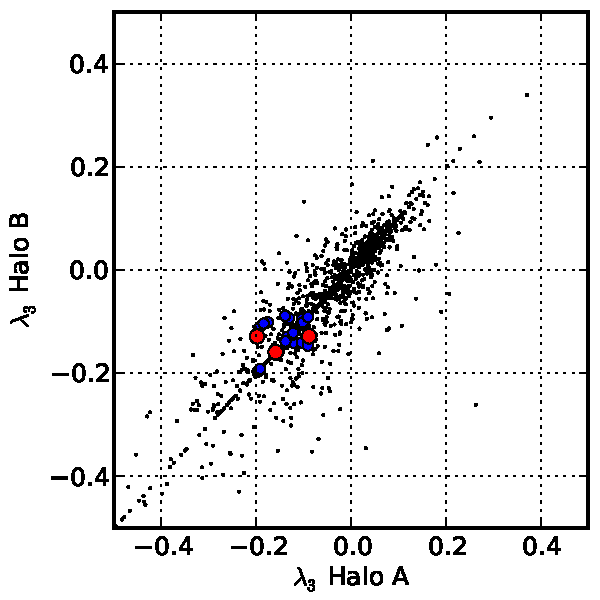
\includegraphics[width=0.46\textwidth]
	{./figures/4_results/CLG_L31_L32.pdf}

	\caption{\small{Comparación entre las distribuciones de los autovalores de 
	la V-web para los dos halos en los sistemas de pares (muestras \textit{LG},
	\textit{CLG} y \textit{IP}).}}
	\label{fig:Lambda_Comparison_Pairs}
\end{figure}
%.........................................................................


Para cuantificar este efecto, en la figura \ref{fig:Lambda_Comparison_Pairs}
son graficadas las distribuciones de cada uno de los autovalores de la V-web
para cada halo de las muestras de pares. La situación ideal, donde ambos
halos comparten una misma celda, correspondería a un línea perfecta 
con pendiente de $45^o$, mientras las situaciones patológicas son responsables 
de dispersiones en las gráficas. Una manera de solucionar esto es disminuir la
resolución de la malla tal que ambos halos estén embebidos en una misma celda, 
pero esto ocasiona una perdida de información del entorno local propio del 
sistema. Debido al suavizado Gaussiano de una celda ($\sim 1 h^{-1}$ Mpc) 
que es aplicado a priori a cada campo de autovalores, la variación de estos 
entre celdas vecinas es menor, tal como es mostrado para la mayoría de 
sistemas \textit{IP} en la gráfica. Teniendo en cuenta esto último y que la 
dinámica local de los pares estará dominada por el halo más masivo, por 
convención será tomada la celda asociada a este halo para la cuantificación
del entorno de todo el sistema.

\
%.........................................................................
%2D Distribution of Vweb eigenvalues in sairs samples
\begin{figure}[htbp]
	\centering
	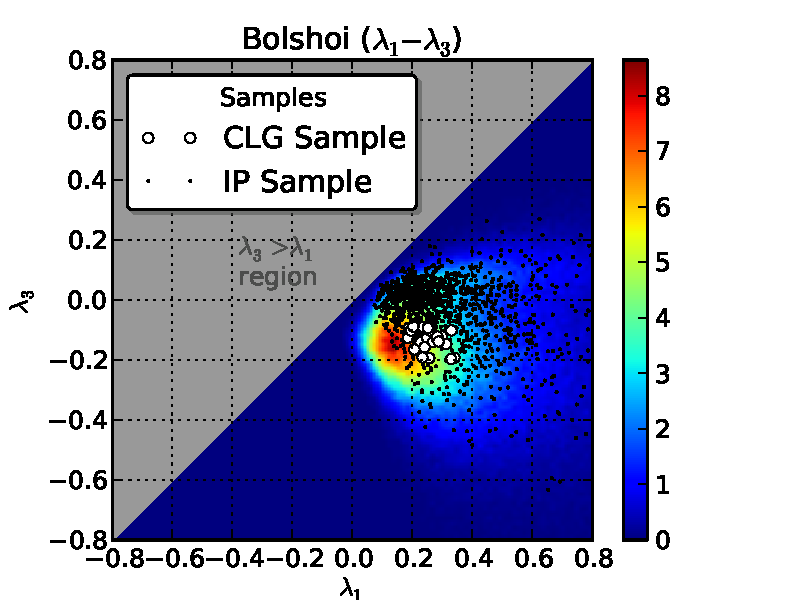
\includegraphics[trim = 0mm 0mm 15mm 0mm, clip, width=0.49\textwidth]
	{./figures/4_results/CLG_Environmet_L1L3.pdf}
	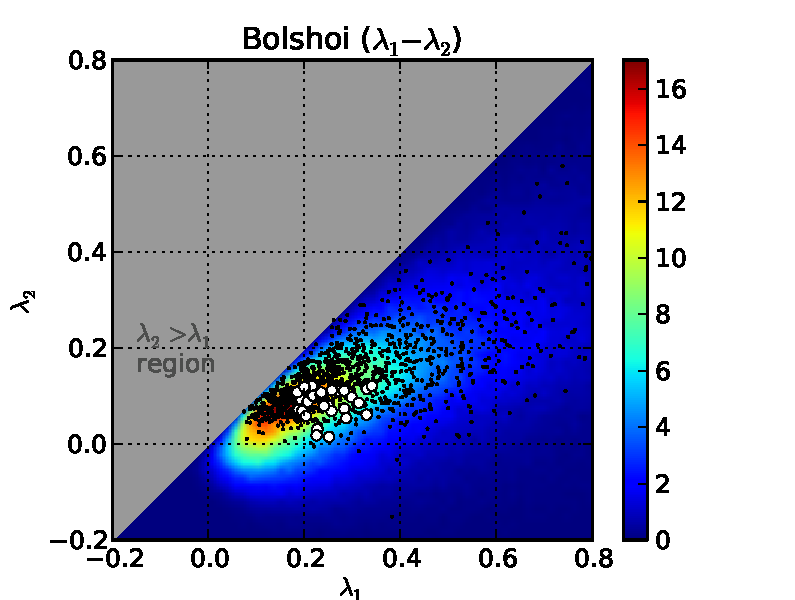
\includegraphics[trim = 0mm 0mm 15mm 0mm, clip, width=0.49\textwidth]
	{./figures/4_results/CLG_Environmet_L1L2.pdf}
	
	\caption{\small{Distribuciones 2D del entorno cosmológico para 
	diferentes muestras, $\lambda_1$--$\lambda_3$ (izquierda) y 
	$\lambda_1$--$\lambda_2$ (derecha). El histograma de fondo, graficado
	en colores, corresponde a la distribución de entorno para todos los 
	halos de Bolshoi (muestra \textit{GH}), su resolución es de $100\times 100$ 
	para el rango mostrado y están normalizados respecto a su área. Los 
	puntos negros corresponden a la distribución de la muestra \textit{IP} 
	y finalmente los puntos blancos a la muestra \textit{CLG}.}}
	\label{fig:2D_Samples_Eigenvalues}
\end{figure}
%.........................................................................


Una vez determinada la forma de cuantificar el entorno de los sistemas de
pares, en la figura \ref{fig:2D_Samples_Eigenvalues} se ilustra la 
distribución de las muestras \textit{GH}, \textit{IP} y \textit{GCL}.
Como fue mostrado en la subsección \ref{subsec:Environment_Properties}, 
la distribución de entorno de los halos en Bolshoi está considerablemente
sesgada respecto a la distribución de las celdas de volumen. A pesar de 
esto y teniendo en cuenta que la construcción de los sistemas de pares se 
hace a partir de los halos, es más interesante realizar comparaciones con las 
distribuciones asociadas a los halos (histogramas de color en la misma figura).
Como fue definido en la subsección \ref{subsec:SampleOfPairsToUse}, la 
muestra \textit{IP} es construida de tal forma que se garantice su
aislamiento gravitacional respecto a halos más masivos, por esta razón hay
dos efectos que compiten en cuanto a la distribución de entorno de estos 
sistemas. En el primero se espera que la abundancia de pares sea más 
favorable en entornos donde la cantidad de halos es mayor, mientras en el
segundo, precisamente la sobreabundancia de halos resulta desfavorable para
los criterios de aislamiento gravitacional. El segundo efecto termina siendo
dominante y produce un sesgo en la distribución de entorno
de la muestra \textit{IP} respecto a la de los halos, mientras que para en 
la muestra \textit{P} el sesgo no se presenta\footnote{Esto 
último no es mostrado en la figura \ref{fig:2D_Samples_Eigenvalues}, pero
es fácilmente calculado.}. 


Para terminar el análisis de la anterior figura, se discute acerca de la 
distribución de entorno para los \textit{CLG} de la simulación Bolshoi. A 
pesar de que esta distribución es construida de forma artificial por 
efecto de selección, es interesante notar que la región en el espacio de 
autovalores que delimita esta muestra es relativamente reducida, indicando 
que los tres grupos locales de las simulaciones CLUES comparten una 
dinámica de entorno local muy similar. Aunque esto último puede ser un 
efecto impuesto a priori por construcción debido al carácter restringido 
de las simulaciones CLUES, no deja de ser interesante el sesgo que esta 
característica produce en la distribución de entorno de los \textit{CLG} 
respecto a los halos y a la muestra \textit{IP}.


Para cuantificar los sesgos producidos en cada muestra respecto a un tipo
de entorno específico (ver figura \ref{fig:ClassificationSchemeTweb}),
en la siguiente figura \ref{fig:Samples_Fraction} se grafican las 
fracciones de objetos en las diferentes regiones. En el rango óptimo del 
valor umbral $0.2\leq \lambda_{th}\leq 0.4$ definido en la subsección 
\ref{subsec:Environment_Properties}, se notan importantes diferencias entre
cada una de las muestras, especialmente para la \textit{CLG}. Como fue 
mencionado anteriormente, el efecto de aislamiento gravitacional produce
un sesgo entre la distribución de entorno de los halos \textit{GH} y de los 
sistemas \textit{IP}, esto puede ser claramente notado para cada una de las 
fracciones en el rango óptimo de $\lambda_{th}$. En el caso de vacíos, la 
fracción dominante de estas dos muestras es la asociada a \textit{IP}, pero 
en el caso de hojas ambas son comparables, y más aún, en la regiones tipo 
filamento y nudo domina la fracción de halos \textit{GH}. Esto indica que
los sistemas de pares aislados \textit{IP} se presentan con mayor 
abundancia en regiones de media o baja densidad de halos, aún así la 
considerable fracción de estos presentes en hojas y filamentos no permite 
asociar un tipo de región de entorno específica para estos sistemas. 
Finalmente, los sistemas \textit{CLG} presentan un importante sesgo 
en comparación a las dos muestras anteriores, siendo de especial interés 
aquella producida respecto a la \textit{IP} debido a que \textit{CLG} es 
una submuestra de esta. De nuevo, apelando al rango óptimo de $\lambda_{th}$,
es posible en este caso asociar tipos de regiones de entorno específicas 
a la muestra \textit{CLG}, estando estos sistemas preferencialmente en 
hojas y vacíos.

\
%.........................................................................
%Number Fraction of each sample in differents type of regions
\begin{figure}[htbp]
	\centering
	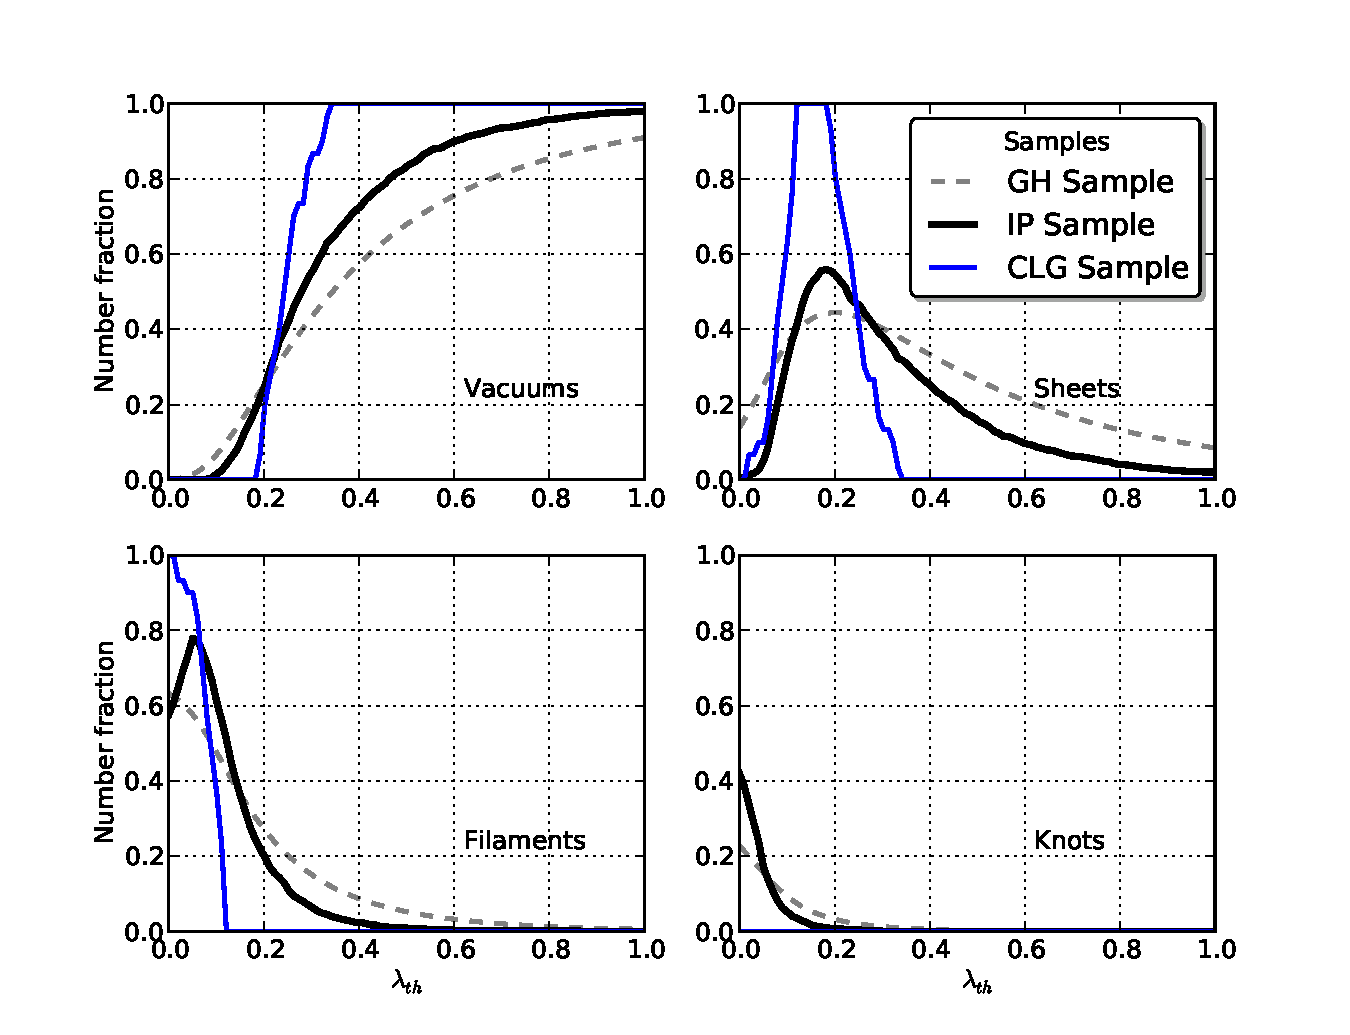
\includegraphics[trim = 8mm 5mm 12mm 12mm, clip, width=0.9\textwidth]
	{./figures/4_results/CLG_Classification_Env.pdf}
	
	\caption{\small{Fracciones de cantidad de objetos en diferentes
	regiones en función del valor umbral $\lambda_{th}$. Para el caso de 
	la muestra \textit{GH} se cuentan número de Halos, mientras que para
	las muestras \textit{IP} y \textit{CLG} número de pares.}}
	\label{fig:Samples_Fraction}
\end{figure}
%.........................................................................


A pesar del esquema de clasificación de regiones usado, las conclusiones 
anteriores dependen de la elección del parámetro $\lambda_{th}$, que aunque
ha sido razonablemente acotado en una región óptima que reproduce la 
impresión visual, no deja de ser un parámetro libre. Para solventar esto se 
introduce el fraccional de anisotropía (FA) con la normalización usada en
\cite{libeskind2013}


%.........................................................................
%Fractional Anisotropy
\eq{eq:FA}
{ FA = \frac{1}{\sqrt{3}}\sqrt{ \frac{ (\lambda_1 - \lambda_3)^2 + 
(\lambda_2 - \lambda_3)^2 + (\lambda_1 - \lambda_2)^2}{ \lambda_1^2 + 
\lambda_2^2 + \lambda_3^2} } }
%.........................................................................


Esta cantidad cuantifica el grado de anisotropía del entorno cosmológico
local, siendo $FA = 1$ una región altamente anisotrópica, mientras
$FA = 0$ un región con alta isotropía, además es independiente de la
elección a priori de algún parámetro libre. Acorde al resultado obtenido por
\cite{libeskind2013}, regiones de baja anisotropía corres\-ponden a nudos
debido a su colapso isotrópico, mientras que regiones de alta anisotropía 
corresponden a vacíos debido a su expansión no uniforme. Para regiones
filamentales y planas el fraccional de anisotropía está distribuido 
de forma extendida en valores intermedios, indicando que la dinámica de
este tipo de entornos es más compleja. Aún así, hay una tendencia a valores
bajos en el caso de filamentos y valores altos para hojas.


%.........................................................................
%Anisotropy Fractional for pairs samples
\begin{figure}[htbp]
	\centering
	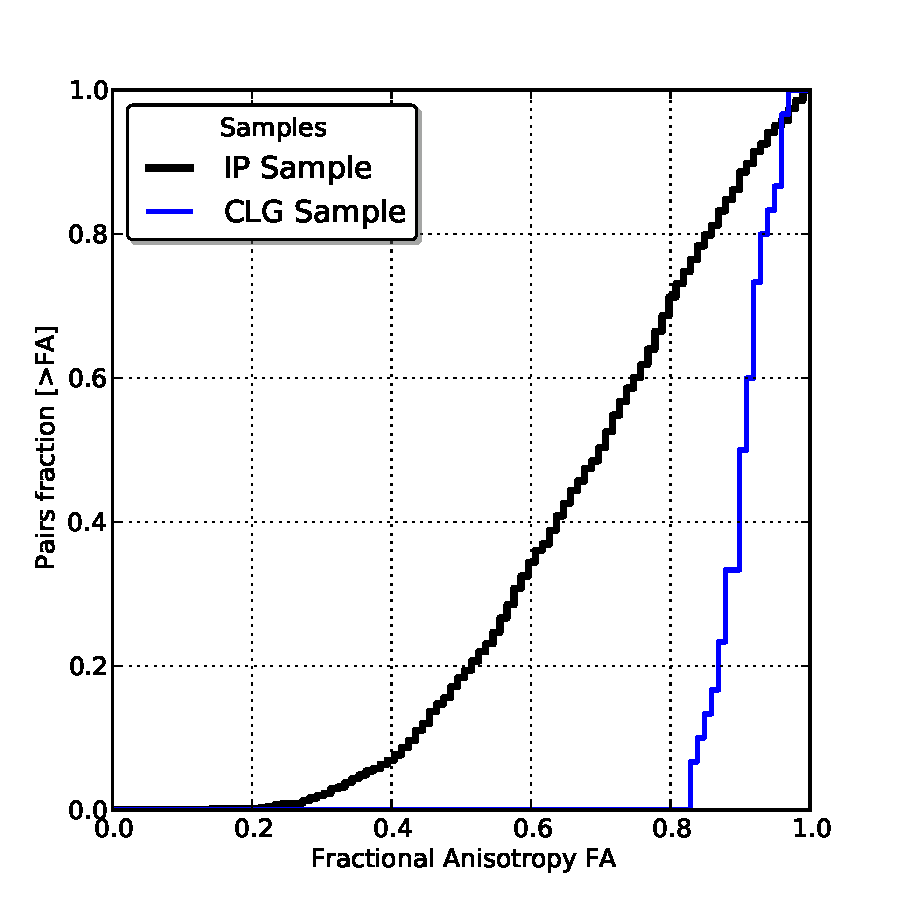
\includegraphics[trim = 0mm 0mm 0mm 10mm, clip, width=0.8\textwidth]
	{./figures/4_results/CLG_FA_Hist.pdf}
	
	\caption{\small{Histograma integrado del fraccional de anisotropía para
	las muestras de pares \textit{IP} y \textit{CLG}.}}
	\label{fig:FA_samples}
\end{figure}
%.........................................................................	


En la figura \ref{fig:FA_samples} son calculados los histogramas integrados
del fraccional de anisotropía para las muestras \textit{IP} y \textit{CLG}.
El primer resultado está asociado a la distribución de los \textit{IP}, 
la cual es altamente homogénea para rangos intermedios (aproximadamente 
$0.4 < FA < 0.9$) como es evidenciado en la pendiente constante del 
histograma. Esto implica que los sistemas \textit{IP} están distribuidos
en zonas de media a alta anisotropía, en concordancia con las fracciones 
encontradas en regiones de vacío, hojas y filamentos. El segundo resultado
es el sesgo obtenido en la distribución de FA de la muestra \textit{CLG}.
A diferencia de los \textit{IP}, esta distribución se encuentra concentrada 
en regiones de alta anisotropía (aproximadamente $0.8 < FA < 1.0$), lo que
confirma finalmente que es posible asociar un tipo de entorno cosmológico a 
los sistemas \textit{CLG} y el cual esta acorde con regiones vacías y 
planas, o en términos de las direcciones definidas en la V-web, regiones 
que se expanden en dos direcciones (asociadas a los autovalores 
$\lambda_2$ y $\lambda_3$), mientras que poseen un ligero colapso/expansión 
en la tercera dirección (asociada al autovalor $\lambda_1$). 


La principal ventaja de usar el fraccional de anisotropía radica en que 
esta cuantifica en un solo valor la dinámica del entorno cosmológico, 
permitiendo establecer un marco de estudio más natural y directo para 
correlaciones de entorno con cantidades fisicas.


	%---------------------------------------------------------------------
	%Pairs Mass
	\subsection{Masa de los \textit{CLG}}
	\label{subsec:CLG_Mass}
	%---------------------------------------------------------------------
	

Como fue demostrado en la subsección \ref{subsec:Halos_Properties}, la 
distribución de masa de los halos es consistente entre las diferentes
simulaciones, por tanto se espera que todas las muestras, a excepción de 
\textit{CLG} que requiere además del entorno cosmológico, sean también
consistentes entre las simulaciones. Para el estudio de las masas de los
sistemas de pares se propone el uso de dos cantidades, la primera es la
masa total del sistema $M_{tot} = M_A + M_B$ y la segunda es la relación 
de las masas $\chi = M_B/M_A$, donde por convención $M_A$ es el halo más 
masivo.


En la siguiente figura \ref{fig:CLG_Mass} se calculan los histogramas 
integrados para la masa total y la razón de las masas. Se toma la muestra
\textit{IP} como muestra de control, además se muestran los valores 
obtenidos para cada uno de los grupos locales en CLUES.


%.........................................................................
%Integrated Mass Fraction
\begin{figure}[htbp]
	\centering
	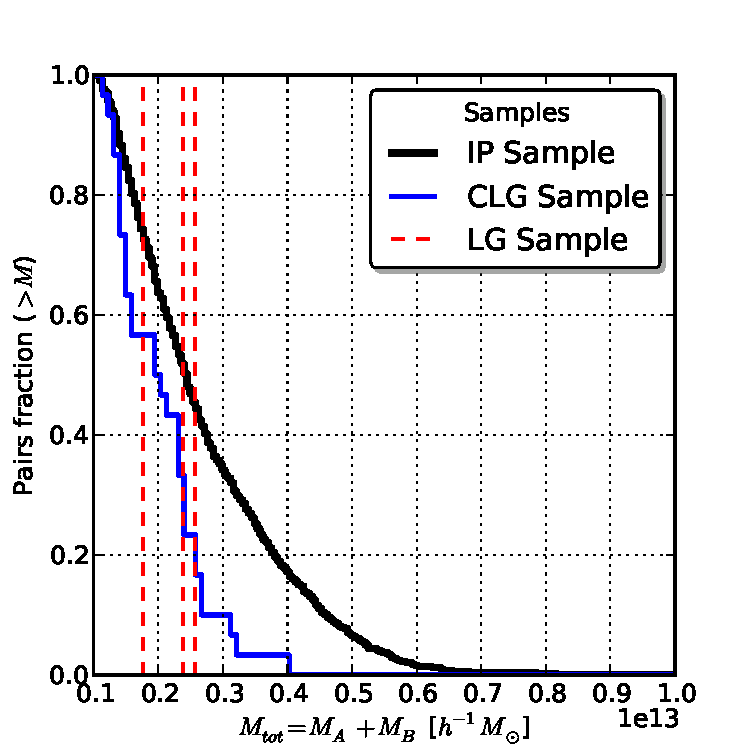
\includegraphics[trim = 0mm 0mm 9.5mm 10mm, clip, width=0.45\textwidth]
	{./figures/4_results/IP_IMF.pdf}
	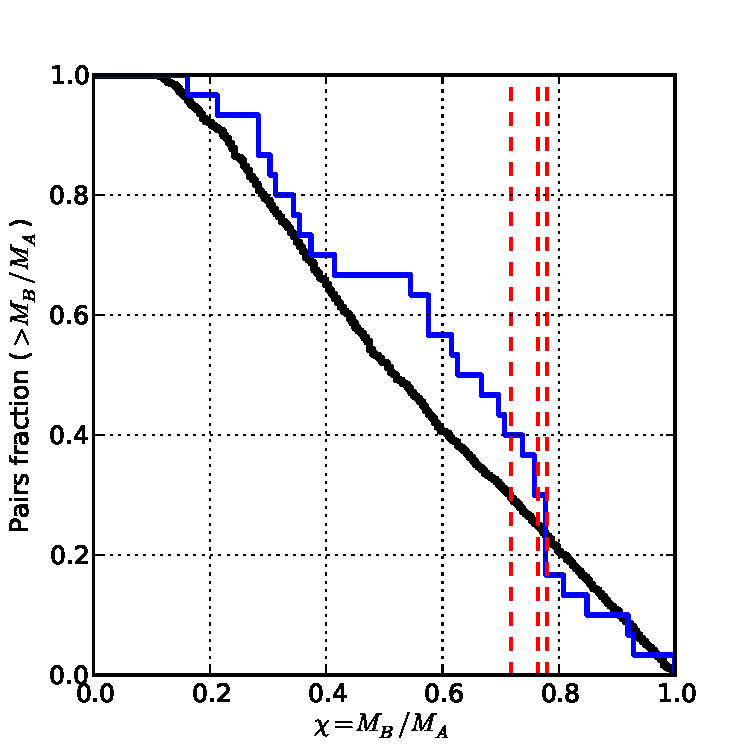
\includegraphics[trim = 0mm 0mm 9.5mm 10mm, clip, width=0.45\textwidth]
	{./figures/4_results/IP_Mass_Ratio.pdf}
	
	\caption{\small{ Funciones de distribución integrada para la masa total
	$M_{A} + M_{B}$ (izquierda) y la razón de las masas $M_B/M_A$ (derecha), 
	de las muestras de pares en Bolshoi. }}
	\label{fig:CLG_Mass}
\end{figure}
%.........................................................................


Una característica interesante de esta figura consiste en los rangos bien 
definidos asociados a la muestra \textit{LG} de CLUES (líneas rojas 
verticales). Esto evidencia que los grupos locales \textit{LG} no solo 
comparten una entorno cosmológico común sino también una distribución de 
masa local. Como posible explicación a esto puede considerase un efecto de 
selección de las muestras en la construcción de las simu\-laciones 
restringidas, mientras que una alternativa optimista sería tomarlo como 
una evidencia de la correlación entre la distribución de masa y el entorno 
local.


Para responder la anterior cuestión se debe analizar la distribución de
los pará\-metros de masa para las demás muestras. En el caso de la masa
total de los \textit{IP}, esta se encuentra distribuida acorde a 
la distribución de masa de los halos (ver figura \ref{fig:IMF}), tal 
como es esperado al no existir ninguna restricción respecto al 
entorno y en el caso de la razón de masas, se obtiene una distribución
completamente homogénea. Ahora, para la muestra \textit{CLG}, la cual se 
espera que sea influenciada por los efectos del entorno, se obtiene una 
distribución de masa total sesgada respecto a la de \textit{IP} y centrada 
aproximadamente en el rango definido por los \textit{LG}. Para la 
distribución de la razón de masas de \textit{CLG} también se encuentra 
un comportamiento uniforme teniendo en cuenta la escasez de datos, 
a pesar de esto hay una aparente sobreabundancia en torno al valor medio 
definido por los \textit{LG}, pero nuevamente no hay suficientes datos 
para concluir una posible relación.

\newpage
%.........................................................................
%Dispersion diagram for pairs mass parameters
\begin{figure}[htbp]
	\centering
	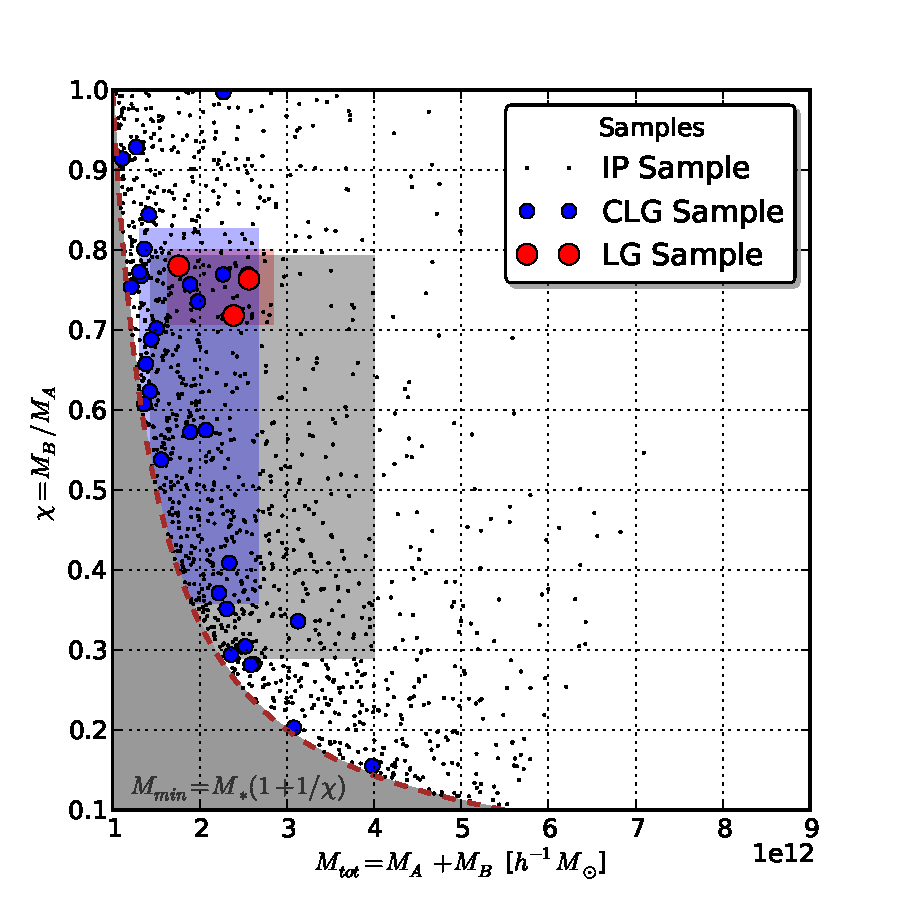
\includegraphics[trim = 0mm 0mm 0mm 10mm, clip, width=0.8\textwidth]
	{./figures/4_results/IP_Mass_vs_Ratio.pdf}
	
	\caption{\small{Diagrama de dispersión de los parámetros de masa 
	definidos ($M_{tot}$,$\chi$) para cada una de las muestras de pares.
	Las regiones cuadradas son construidas a partir del valor medio y la
	desviación estándar de la muestra del mismo color.
	La región gris en la parte inferior izquierda corresponde a un corte
	impuesto artificialmente con el rango mínimo de masa de los halos 
	tomados $M_*$ para construir las muestras de pares.}}
	\label{fig:Dispersion_Mass_CLG}
\end{figure}
%.........................................................................


En la figura \ref{fig:Dispersion_Mass_CLG} se muestra un diagrama de 
dispersión para los parámetros de masa de las muestras de pares. Las 
regiones cuadradas representan el valor medio más o menos una desviación
estándar para las parámetros marcados en cada eje, lo que permite comparar
gráficamente las distribuciones. De esta comparación se confirma que el 
criterio de construcción de la muestra \textit{CLG} selecciona masas de 
pares $M_{tot}$ consistente con las masa de los \textit{LG} en las simulaciones 
restringidas, mientras que no hace ninguna selección respecto a la razón 
de masas $\chi$.


Finalmente, con el objetivo de responder si existe un posible efecto de 
entorno en la selección de la masa total obtenida para la muestra 
\textit{CLG}, se calcula en la siguiente figura \ref{fig:CLG_FA_Mass} 
diagramas de correlación entre el fraccional de anisotropía y los parámetros 
de masa.

\
%.........................................................................
%Correlation Mass-FA
\begin{figure}[htbp]
	\centering
	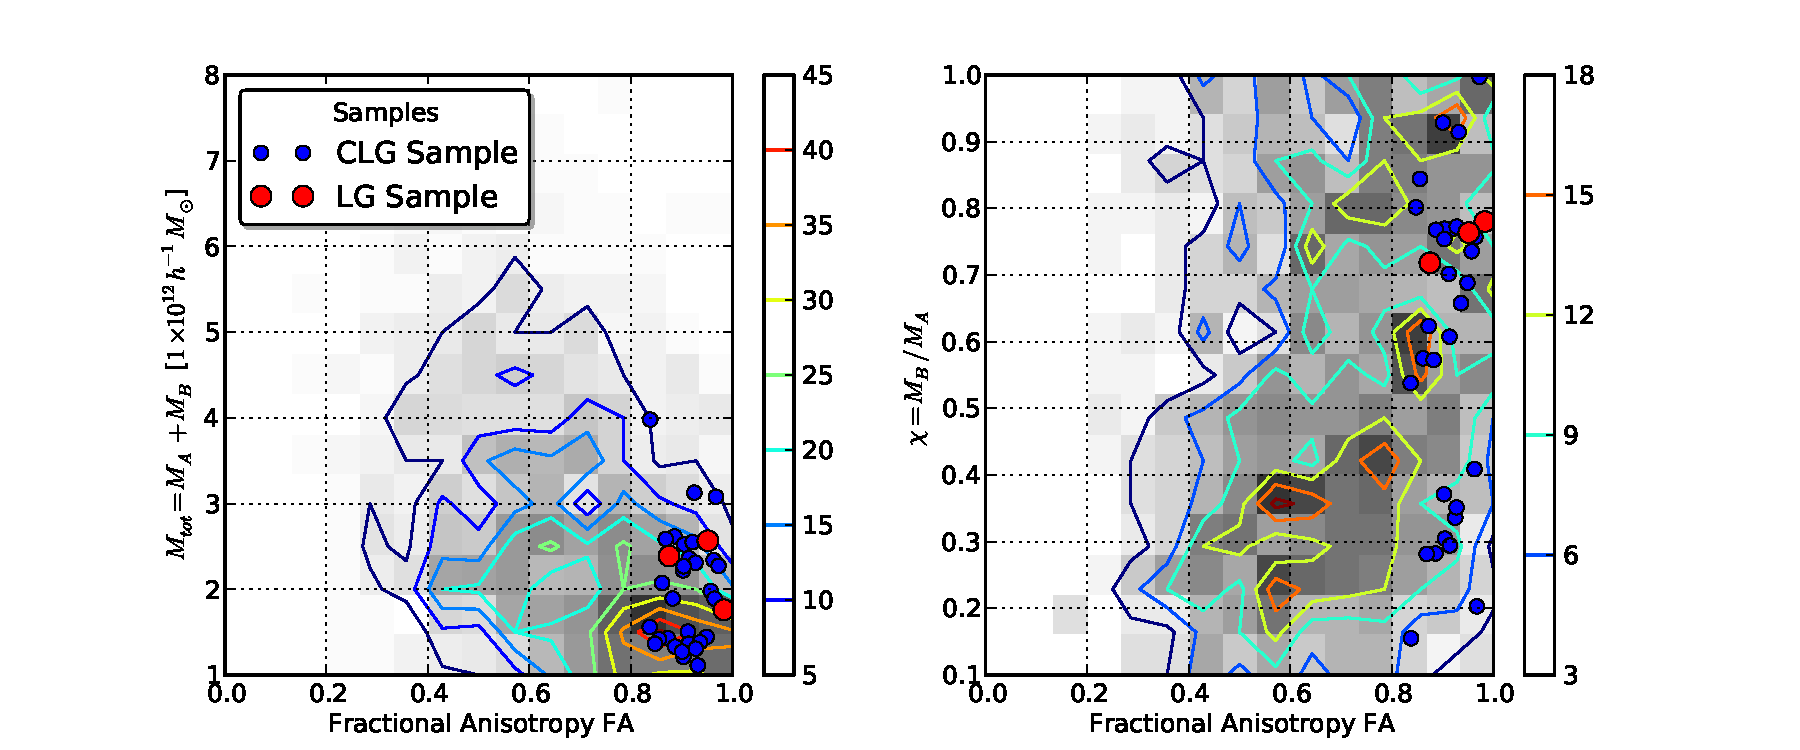
\includegraphics[trim = 25mm 0mm 35mm 10mm, clip, width=1.0\textwidth]
	{./figures/4_results/CLG_FA_Mass.pdf}
	
	\caption{\small{Diagramas de dispersión para el fraccional de 
	anisotropía respecto a los parámetros de masa. El mapa de fondo y las
	curvas de contorno corresponden a número de pares de la muestra 
	\textit{IP}.}}
	\label{fig:CLG_FA_Mass}
\end{figure}
%.........................................................................
\

En el caso de la masa total $M_{tot}$ de la muestra \textit{IP}, puede 
notarse que pares con bajos valores de masa están preferencialmente en 
regiones de alta anisotropía, mientras que pares de masa más alta en 
regiones de anisotropía intermedia. Esto puede ser considerado como una 
correlación de entorno para la muestra \textit{IP} respecto a la masa total, 
de lo cual se concluye que el criterio de selección de la muestra \textit{CLG}
a partir del entorno de los \textit{LG} hace un corte para pares de baja 
masa.


Para la razón de las masas $\chi$ se nota una distribución más dispersa 
para la muestra \textit{IP}, a pesar de esto se nota una sobreabundancia 
de pares con valores de $\chi$ bajos en zonas de anisotropía media, 
mientras que en regiones de alta anisotropía se presentan valores más altos
de $\chi$. Esto es consistente con la selección realizada en la muestra
\textit{CLG}, para la cual aproximadamente el $66\%$ de los pares tienen
un valor $\chi>0.5$. De esto puede intuirse una posible correlación entre
el entorno y el valor $\chi$ de los pares, aún así, debido a la alta 
dispersión de la distribución y la poca cantidad de datos, no puede 
concluirse nada al respecto.
\newpage

	%---------------------------------------------------------------------
	%Angular momentum and energy
	\subsection{Distribuciones de Energía y Momentum Angular}
	\label{subsec:AngularMomentumAndEnergy}
	%---------------------------------------------------------------------


La energía y el momentum angular constituyen otras propiedades físicas de
interés para los sistemas de pares, estas son definidas acá a partir de las
siguiente expresiones


%.........................................................................
%Energy of Pairs
\eq{eq:EnergyPairs}
{ e_{tot} = \frac{1}{M_A + M_B}\cor{ \frac{1}{2}\pr{ M_A v_A'^2 + M_B v_B'^2 } 
 - G\frac{M_A M_B}{| \bds r_A' - \bds r_B' |}}
 }
%.........................................................................


%.........................................................................
%Angular Momentum of Pairs
\eq{eq:AMomentumPairs}
{ \bds L_{orb} = \frac{1}{M_A + M_B}\cor{ M_A\bds r_A' \times \bds v_A' + 
M_B\bds r_B' \times \bds v_B' }}
%.........................................................................
donde $\bds r_i'$ es la posición comóvil del halo $i$ y $\bds v_i'$ es la 
velocidad total\footnote{Velocidad total debido a que se incluye la velocidad 
peculiar y el flujo de Hubble respecto al centro de masa del sistema, así 
$\bds v_i' = \bds v_{pec,i} + H_0 \bds r_i'$. } respecto al centro de 
masa del par.


%.........................................................................
%Energy-AMomentum Dispersion
\begin{figure}[htbp]
	\centering
	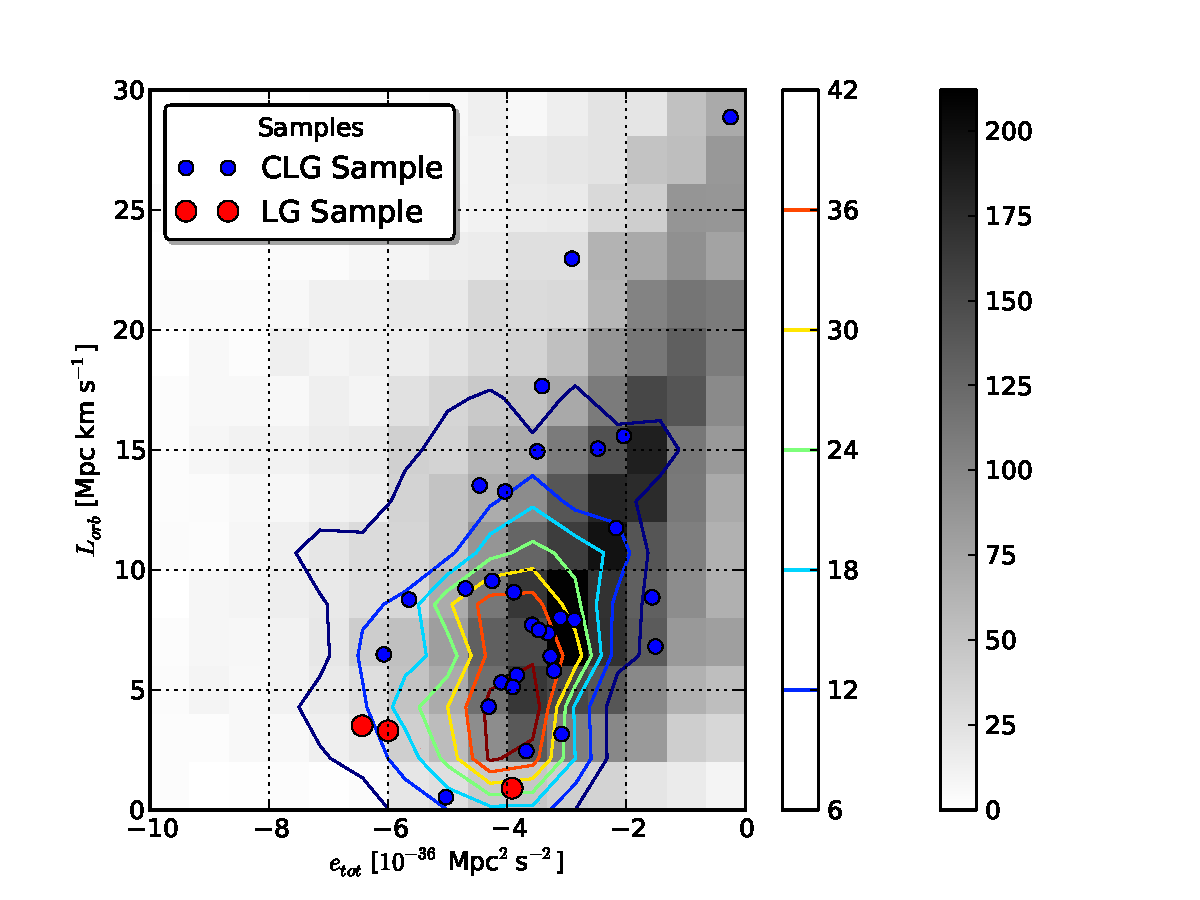
\includegraphics[trim = 8mm 0mm 25mm 10mm, clip, width=0.8\textwidth]
	{./figures/4_results/CLG_E_vs_L.pdf}
	
	\caption{\small{Diagrama de dispersión para la energía total y el 
	momentum angular orbital de los sistemas de pares. El mapa de fondo
	corresponde a la distribución de la muestra \textit{P}, mientas las
	líneas de contorno a la distribución de la muestra \textit{IP}, en 
	ambos casos los valores corresponden al número de pares. }}
	\label{fig:CLG_E-L}
\end{figure}
%.........................................................................	


En la figura \ref{fig:CLG_E-L} se muestran las distribuciones de energía 
total específica y momentum angular orbital específico para las diferentes 
muestras. Lo primero que puede ser notado es un significativo sesgo entre
la distribución de los \textit{IP} respecto a los \textit{P}, lo que 
demuestra que el criterio de aislamiento gravitacional definido en la 
subsección \ref{subsec:SampleOfPairsToUse} selecciona un rango de energía 
y momentum angular más bajo que en los pares generales, siendo así estos 
sistemas gravitacionalmente más ligados. En el caso de la muestra 
\textit{CLG}, su distribución parece seguir la de los \textit{IP},
no habiendo así una aparente selección por la condición entorno. Por último,
es interesante observar nuevamente que las propiedades asociadas a la
muestra \textit{LG} poseen valores muy cercanos, indicando así que
representan un tipo de sistema bien definido, aunque como ha sido mencionado,
esto puede ser efecto de selección en la construcción de CLUES.

\
%.........................................................................
%Correlation Energy, L_orb-FA
\begin{figure}[htbp]
	\centering
	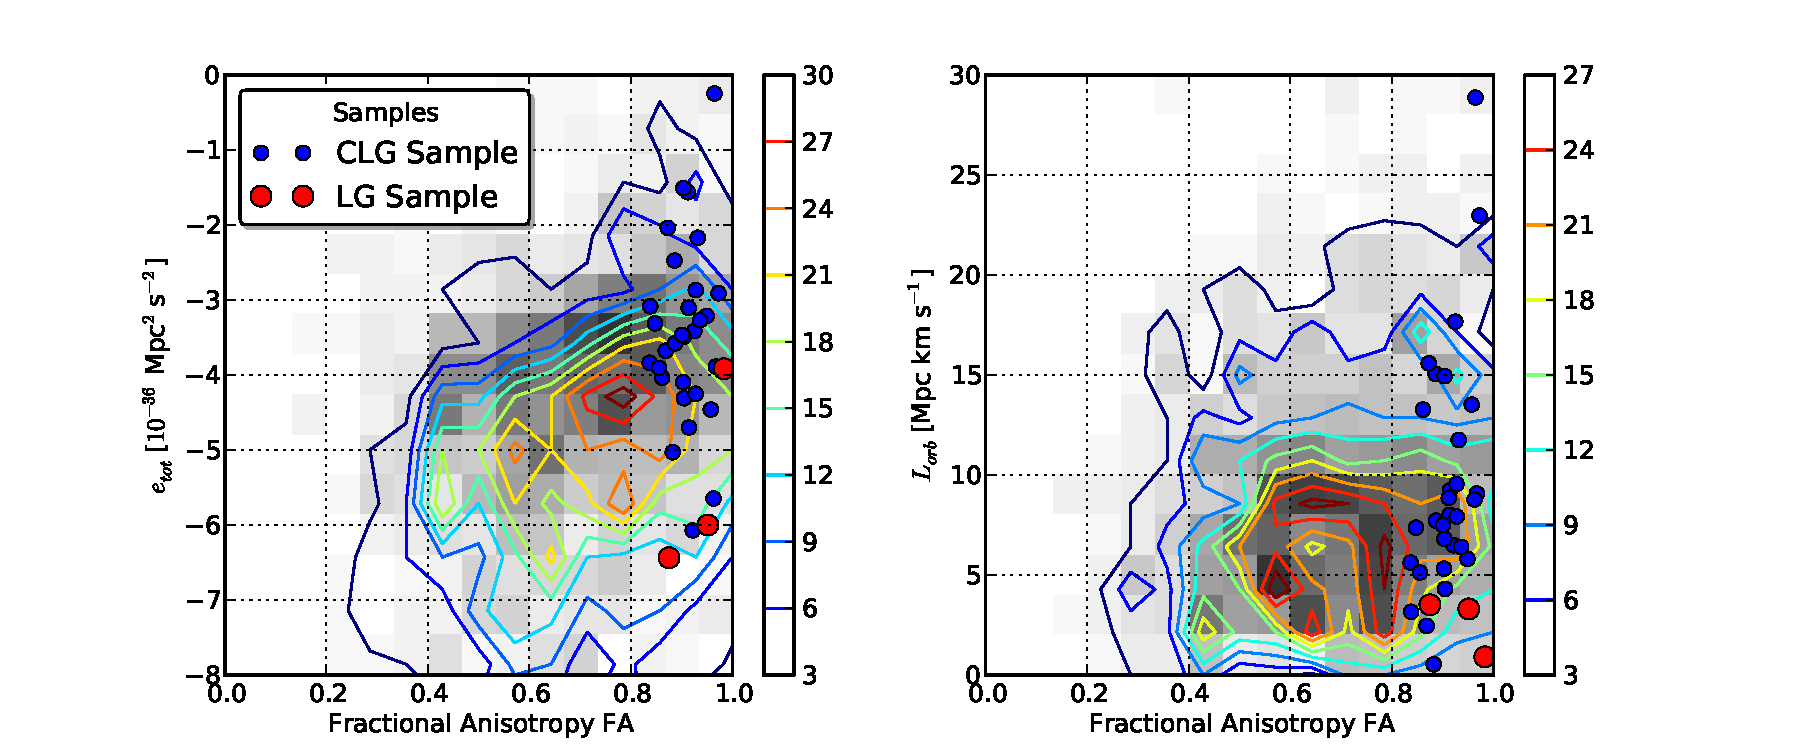
\includegraphics[trim = 20mm 0mm 35mm 10mm, clip, width=1.0\textwidth]
	{./figures/4_results/CLG_FA_E-L.pdf}
	
	\caption{\small{Diagramas de dispersión para el fraccional de 
	anisotropía respecto a la energía y el momentum angular. El mapa de 
	fondo y las curvas de contorno corresponden a número de pares de 
	la muestra 	\textit{IP}.}}
	\label{fig:CLG_FA_E-L}
\end{figure}
%.........................................................................


En la figura \ref{fig:CLG_FA_E-L} se calculan diagramas de correlación de
la energía y el momentum angular con el fraccional de anisotropía con el 
objetivo de determinar posibles correlaciones. En el caso de la energía
específica, sistemas de pares \textit{IP} con mayor energía (menos ligados) 
parecen estar mayoritariamente en zonas de alta anisotropía, mientras que
sistemas de menor energía (más ligados) están en zonas de anisotropía media,
lo que muestra una correlación entre estas dos cantidades. Para sistemas
\textit{CLG}, la selección a partir del entorno parece sesgar su 
distribución de energía a valores más altos que la distribución media de los
\textit{IP}, lo que es consistente con la correlación encontrada. En este
caso, los sistemas \textit{LG} parecen no seguir esta correlación, teniendo
valores mucho más bajos de energía que lo esperado. Finalmente, para la 
distribución de momentum angular específico no existe ninguna correlación 
clara, siendo cualquier valor $L_{orb}$ de los pares igualmente probable 
en el espectro de posibles entornos para estos sistemas.


	
	%---------------------------------------------------------------------
	%Alineación del momentum angular
	\subsection{Alineación del Momentum Angular}
	\label{subsec:AngularMomentumAlineation}
	%---------------------------------------------------------------------
	
	
Finalmente la última propiedad analizada para los sistemas de pares es su
alineación respecto al entorno cosmológico, para esto se define el ángulo
$\phi_i$ como el formado entre el autovector $\bds u_{\lambda i}$ de la
V-web y el momentum angular del par $\bds L_{orb}$.

	
%.........................................................................
%CLG Alineation
\begin{figure}[htbp]
	\centering
	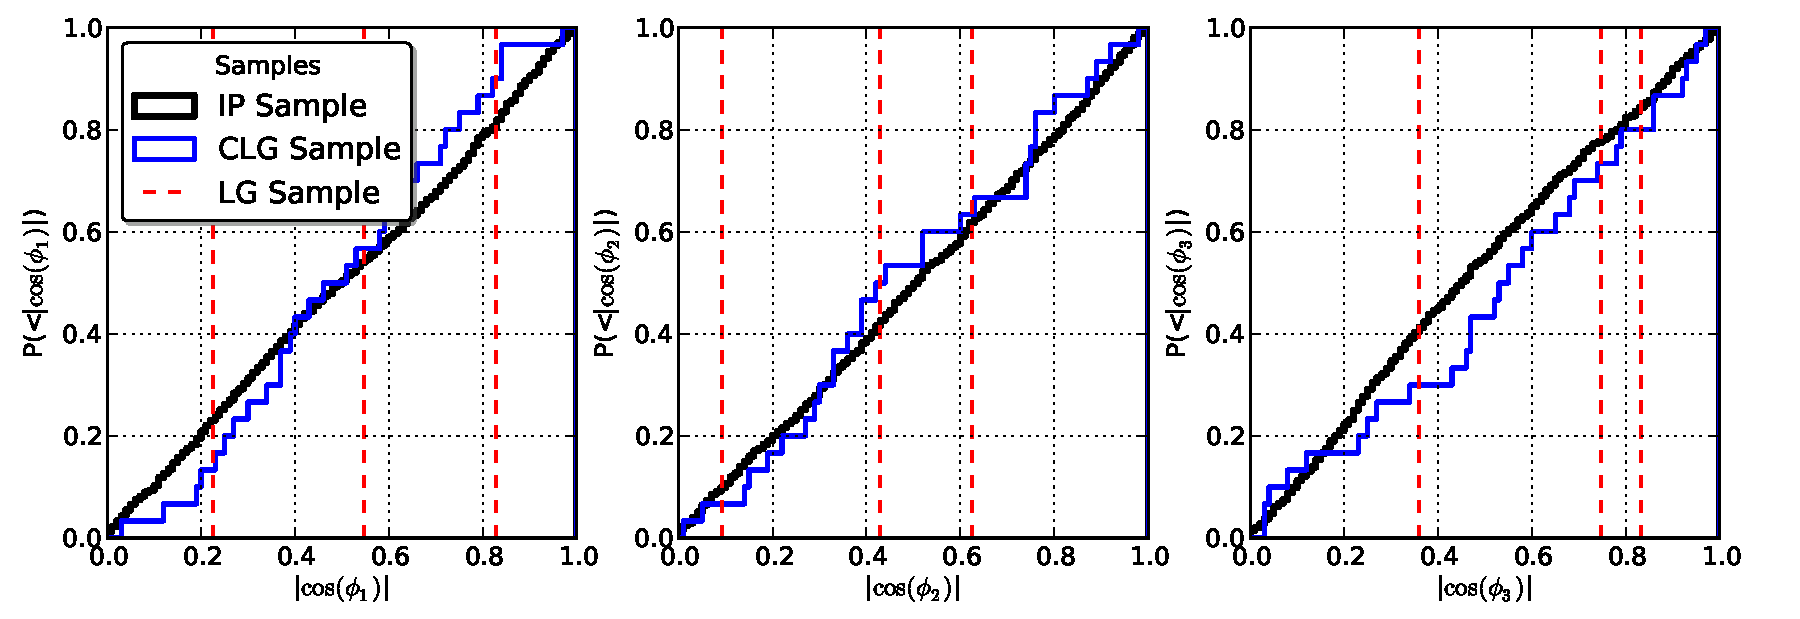
\includegraphics[trim = 0mm 0mm 5mm 0mm, clip, width=1.0\textwidth]
	{./figures/4_results/CLG_Alineation.pdf}
	
	\caption{\small{Histogramas integrados para el ángulo formado entre el 
	momentum angular de los pares, el cual determina el plano orbital, y
	cada uno de los autovectores definidos por la V-web en el entorno
	cosmológico. Se realiza para cada las muestras de pares \textit{CLG} y 
	\textit{IP}, mientras que los grupos locales de CLUES son ilustrados 
	con las líneas rojas punteadas.}}
	\label{fig:CLG_Alineation}
\end{figure}
%.........................................................................
	

En la figura \ref{fig:CLG_Alineation} se calculan los histogramas 
integrados para cada uno de los angulos $\phi_i$ definidos. Como puede 
notarse, las muestras \textit{CLG} y \textit{IP} son homogéneas respecto
a los tres valores, indicando que no hay una alineación preferida respecto
al entorno cosmológico. Esto también se evidencia en los valores calculados
de los \textit{LG} de las simulaciones restringidas.


%*************************************************************************



	
%*************************************************************************
%Conclusions
\section{Conclusiones}
\label{sec:Conclusions}


Esta sección está dedicada a compilar los principales resultados obtenidos
en este capítulo. Estos serán enumerados y discutidos acorde al órden en
que fueron obtenidos.


%.........................................................................
%Main Results
\begin{enumerate}
\item[\textbf{1.}] La construcción de la muestra \textit{IP} fue 
inicialmente propuesta en \cite{forero2011} con el objetivo de reproducir
sistemas tipo grupo local. A pesar de esto, el número de estos sistemas 
encontrados en la simulación Bolshoi es mucho mayor al que se espera acorde
a la abundancia de \textit{LG} en simulaciones restringidas. El método 
propuesto para la selección de la muestra \textit{CLG} en Bolshoi a partir 
del entorno cosmológico de los \textit{LG}, produce un número de sistemas 
que concuerda con los encontrados en la simulaciones restringidas, escalando 
apro\-ximadamente como el volumen de las simulaciones. Más aún, aplicando 
este mismo método en las simulaciones restringidas se halla una muestra
con un tamaño similar a la \textit{LG}.


\item[\textbf{2.}] A partir de los valores medios de densidad en las 
diferentes regiones del entorno cosmológico (figura \ref{fig:Vol_Fraction})
se propone un esquema para la elección de un rango óptimo del parámetro
$\lambda_{th}$ de la V-web con el objetivo de reproducir la 
apariencia visual de la red cósmica. Este está basado en la 
minimización de la densidad media en las regiones de vacío debido a que
son las dominan la apariencia del campo de densidad a gran escala. Con
esto se garantiza que las regiones vacías no invadan regiones de más alta
densidad, que en principio deben ser clasificadas como hojas o filamentos.
Este método da un rango de valores óptimos aproximadamente igual para 
todas las simulaciones usadas ($0.2 \leq \lambda_{th} \leq 0.4$), además
reproduce adecuadamente la apariencia visual (ver figura 
\ref{fig:Vweb_Comparison} para $\lambda_{th} = 0.3$). A pesar de esto, 
este parámetro sigue siendo libre y no es viable usar un esquema de 
clasificación basado en este para determinar correlaciones con propiedades
físicas, en vez de esto se introduce el fraccional de anisotropía 
con la normalización usada en \cite{libeskind2013}.


\item[\textbf{3.}] La distribución del entorno cosmológico de las 
simulaciones Bolshoi y CLUES difieren, existiendo un cambio de densidad 
media muy pronunciado entre regiones de vacío y filamentos en Bolshoi, 
mientras que es mucho más suave en las CLUES. A pesar de esto, las 
fracciones de volumen asociadas a cada tipo de entorno son aproximadamente 
iguales para ambas simulaciones en el rango óptimo determinado para 
$\lambda_{th}$. A pesar de esto, se espera que la dinámica local 
caracterizada por la V-web sea independiente de la estructura global 
de la distribución de entorno, lo cual valida el esquema de selección 
de la muestras \textit{CLG} en Bolshoi.


\item[\textbf{4.}] El método de construcción de los 
\textit{CLG} selecciona un entorno cosmológico común para estos 
sistemas, siendo preferidas zonas de vacío y hojas no muy planas.
Estas regiones presentan una alta anisotropía, cuantificada por el 
fraccional de anisotropía FA. En el caso de los sistemas \textit{IP},
estos se encuentran en zonas de media a alta anisotropía, asociadas 
a valores de baja densidad, contrario a los halos que están en zonas 
más densas y menos anisotrópicas como filamentos y nudos, aún así 
la distribución de entorno de los \textit{IP} es amplia y no pueden
ser asociados a un tipo de entorno específico. El sesgo producido
entre los \textit{IP} y los halos generales se debe al criterio
de aislamiento gravitacional usado para construir los \textit{IP},
esto hace que zonas con mayor densidad de halos sean menos aptas por
la alta influencia gravitacional.


\item[\textbf{5.}] Se encuentra una correlación entre la masa total de 
los pares de la muestra \textit{IP} y el fraccional de anisotropía del 
entorno, donde masas mayores son más abundantes en regiones de 
anisotropía media mientras masas menores se presentan con mayor 
frecuencia en zonas de alta anisotropía. Esto implica que la selección
de entorno realizada en los \textit{CLG} reproduce un rango de masa menor.
En el caso de la razón de masa, no se encuentra ninguna correlación 
significativa con el entorno, aún así se nota una ligera sobreabundancia 
de razones de masa mayores en regiones más anisotrópicas, pero es 
necesaria más estadística para poder ser algo concluyente.


\item[\textbf{6.}] Se halla un correlación para la energía específica
de los sistemas \textit{IP} respecto al entorno, obtiendo valores más
altos en regiones más anisotrópicas y valores bajos en regiones de 
anisotropía media. Esta correlación parece seleccionar un rango de 
energía para los sistemas \textit{CLG}, aunque esta no es consistente
con los valores obtenidos de los \textit{LG}. Para el momentum angular
no se encuentra ninguna correlación con el entorno.


\item[\textbf{7.}] Finalmente se encuentra que no existen alineaciones
privilegiadas entre el momentun angular de los pares \textit{CLG} (o de 
su plano orbital) y las direcciones de los autovectores de la V-web.


\end{enumerate}
%.........................................................................


%*************************************************************************